% Data sythesis using the Robinson/Freyer/Hindriks model - Top Level
% Written by Christopher Thomas.

\documentclass[letterpaper,11pt]{report}
\usepackage[letterpaper]{geometry}
\usepackage{graphicx}
\usepackage{verbatim}
\usepackage{placeins}
\usepackage{longtable}
% Needed for "mathbb" (outline bold).
%\usepackage{amsfonts}

\geometry{nohead,footskip=0.3in,margin=0.75in}

% Force my paragraph style, darnit.
\usepackage{indentfirst}
\setlength{\parskip}{\baselineskip}

% NOTE - "\thispagestyle" is used for part and chapter beginning pages, and
% overrides \pagestyle. Redefine it to be harmless.
% NOTE - The canonical solution ("\pagenumbering{gobble}") resets the page
% counter whenever it's used.
\renewcommand{\thispagestyle}[1]{}

% Custom macros.
\newcommand{\fixme}[1]{\textbf{FIXME: #1}}

\newcommand{\figdef}[3]
{\begin{figure}[htb]
\begin{center}#1\end{center}
\caption{#2}\label{#3}\end{figure}}

% NOTE - This was [hb].
\newcommand{\tabdef}[3]
{\begin{table}[htb]
\begin{center}#1\end{center}
\caption{#2}\label{#3}\end{table}}

% Document body.
\begin{document}
%
% Title page.
%
\pagestyle{empty}

\begin{center}
%
\vspace*{1in}
{\huge Data Synthesis Using the Extended Robinson Model} \\
{\footnotesize Written by Christopher Thomas -- \today.}
%
\vspace*{1.5in}\\
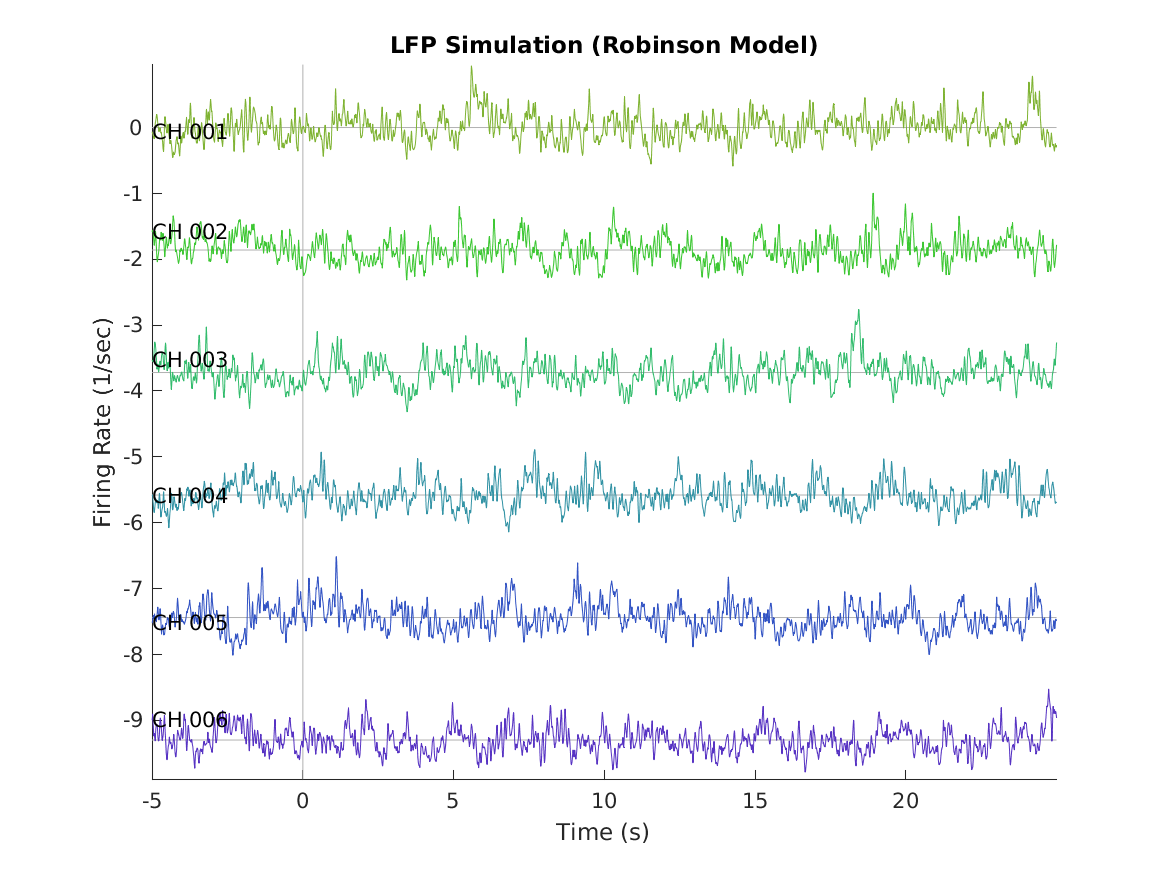
\includegraphics[width=5in]{plots/20231205/lfp-simulation-robinson-model}
%
\end{center}
%
\vfill
{\tiny \input{../LICENSE.md}}
%
\clearpage
%
%
% Front matter.
%
\pagestyle{plain}
\pagenumbering{roman}
\setcounter{page}{1}
%
\tableofcontents
%
\clearpage
%
%
% Document parts.
%
\pagestyle{plain}
\setcounter{page}{1}
\pagenumbering{arabic}
%
% Data sythesis using the Robinson/Freyer/Hindriks model - Overview
% Written by Christopher Thomas.

\chapter{Overview}
\label{sect-over}

\fixme{Edit this.}

This document describes the models used for synthesizing proxy neural
activity using the ``\texttt{nlSynth\_}'' family of library functions.

These functions are primarily intended to produce realistic-looking signals
with known qualities to test analysis scripts with. That said, these models
are drawn from publications where they were used to provide insight into
the functioning of brain networks, so using these functions for such
research is an additional use-case.

Chapter \ref{sect-robinson} describes the neural model presented in
Robinson 2002 (and elaborated on in Freyer 2011 and Hindriks 2023). This
is a model of average firing rates of multiple neural populations in the
cortex and thalamus, with feedback connections that drive noise-excited
oscillations.

\fixme{Other models go here once they're added.}

%
% This is the end of the file.

% Neuroloop utilities - Synthesis model guide - Robinson model
% Written by Christopher Thomas.

\chapter{Robinson Model}
\label{sect-robinson}

The model presented in Robinson 2002 (hereafter ``the Robinson model'')
provides a series of differential equations relating the firing rates of
multiple neural populations in the cortex and thalamus. Feedback between
these regions drives noise-excited oscillations.

The most relevant references are:
\begin{itemize}
\item Robinson 2002 -- Describes the model, finds steady-state points, and
analyzes perturbations around those points to find oscillation modes.
\item Freyer 2011 -- Describes an extension to the model where noise is
modulated by the network's own output, providing a closer match to the
distribution of oscillation modes in biological data.
\item Hindriks 2023 -- Describes an extension to the model that adds multiple
independent copies of the Robinson and Freyer model, with coupling between
instances. This is used to model co-oscillation of different brain regions
in biological data.
\end{itemize}
(See Section \ref{sect-robinson-refs} for citations.)

%
%
\section{Model Description}
\label{sect-robinson-model}

A diagram of the Robinson model with the extensions from Freyer 2011 and
Hindriks 2023 is shown in Figure \ref{fig-robinson-diagram}. To distinguish
this from the Robinson 2002 model, this will be referred to as ``the
extended Robinson model''.

\figdef{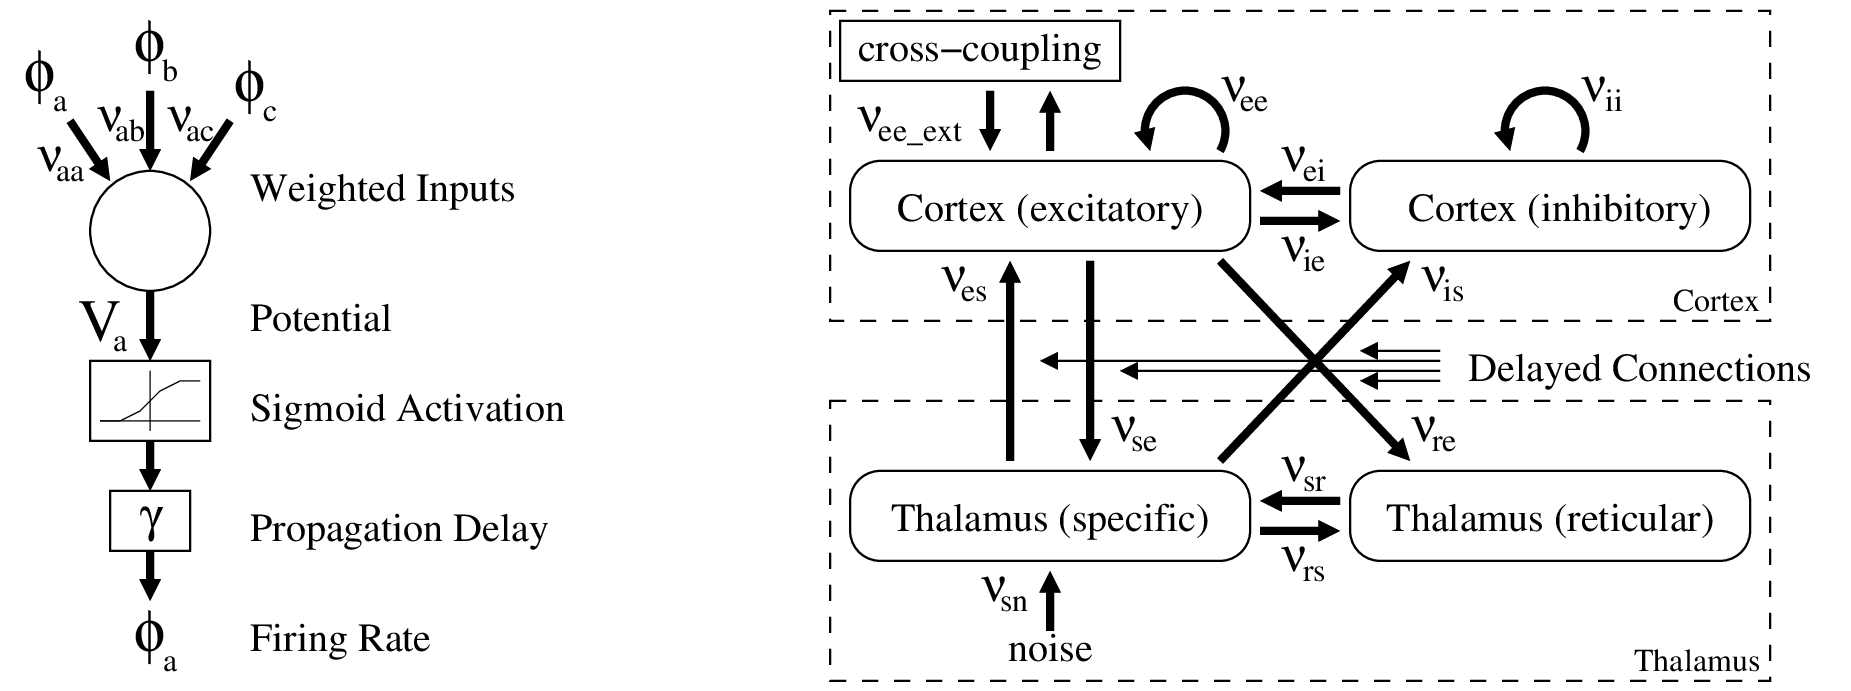
\includegraphics[width=0.9\columnwidth]{figures/robinson-model}}
{Extended Robinson model diagram, showing the neuron population model
(left) and the population interactions (right).}{fig-robinson-diagram}

The neural population model is described in Equations
\ref{eq-robinson-potential}, \ref{eq-robinson-sigmoid} and
\ref{eq-robinson-gamma}.
%
Per Equation \ref{eq-robinson-potential}, a weighted sum of input firing
rates $\phi_b(t)$ is used to generate the cell body potential $V_a(t)$. A
single dot indicates the first time derivative, and a double dot indicates
the second time derivative. The parameters $\alpha$ and $\beta$ are the
inverse of the membrane potential fall time and rise time, respectively.
The coupling parameter $\nu_{ab}$ is the strength of the connection from
region $b$ to region $a$ (zero if no connection, negative if inhibitory).

\textbf{NOTE:} A delay is manually applied to some of the $\phi_b$ signals
before this summation to reflect signal propagation time between the cortex
and thalamus (per Robinson 2002), and to reflect cross-coupling delays
within the cortex populations (per Hindriks 2023).

\begin{equation}
\left ( \frac{1}{\alpha \beta} \right ) \ddot{V}_a(t)
+ \left ( \frac{1}{\alpha} + \frac{1}{\beta} \right ) \dot{V}_a(t)
+ V_a(t) = \sum_b \nu_{ab} \phi_b(t)
\label{eq-robinson-potential}
\end{equation}

Per Equation \ref{eq-robinson-sigmoid}, the cell body potential $V$ is fed
into a sigmoid activation function, to represent the collective action of
many neurons with varying firing thresholds. The mean firing threshold is
$V_{th}$ and the standard deviation of the threshold is $\sigma_{th}$.
This follows the convention of Freyer 2011; Robinson 2002 defined a
related parameter $\sigma'_{th} = \frac{\sqrt{3}}{\pi} \sigma_{th}$ to
simplify the activation equation (Equation \ref{eq-robinson-sigmoid-prime}).

\begin{equation}
Q(V) = \frac{Q_{max}}
{1 + e^{- \left ( \frac{\pi}{\sqrt{3}} \right )
\left ( \frac{ V - V_{th}}{\sigma_{th}} \right )}}
\label{eq-robinson-sigmoid}
\end{equation}

\begin{equation}
Q(V) = \frac{Q_{max}}
{1 + e^{- \left ( \frac{ V - V_{th}}{\sigma'_{th}} \right )}}
\label{eq-robinson-sigmoid-prime}
\end{equation}

Per Equation \ref{eq-robinson-gamma}, the local firing rate $Q$ is
propagated with damping and finite delay to give the non-local firing rate
$\phi$. A single dot indicates the first time derivative, and a double dot
indicates the second time derivative. Per Robinson 2002, local propagation
delay is assumed to only be relevant within the cortex, and
$\gamma = \infty$ is assumed elsewhere. Per Freyer 2011, this further only
applies to the excitatory neuron populations in the cortex.

\begin{equation}
\left \{
\begin{array}{rcl}
\frac{1}{\gamma^2} \ddot{\phi}(t) + \frac{2}{\gamma} \dot{\phi}(t) + \phi(t)
= Q(t) & ~~ & \mathrm{Cortex ~ excitatory ~ neurons.} \\
\phi(t) = Q(t) & ~~ & \mathrm{All ~ other ~ populations.} \\
\end{array}
\right .
\label{eq-robinson-gamma}
\end{equation}

Noise is injected into the model as $\phi_n$, and is described by Equation
\ref{eq-robinson-noise}. Per Freyer 2011, there are three components:
constant, additive, and multiplicative. Multiplicative noise (noise
modulated by $\phi_e$) is important for broadening the distribution of
peak power levels of transient oscillations at frequencies above the
fundamental oscillation mode of the cortex/thalamus loop.

In Equation \ref{eq-robinson-noise}, $\phi_n$ is the noise coupled to
the thalamus via $\nu_{sn}$, $\mu_n$ is the constant noise component
(background firing rate), $\sigma_n$ is the standard deviation of the
independent component of the noise, and $\chi$ is a scaling parameter
(per Freyer 2011) such that $\sigma_n \chi$ is the standard deviation of
the component of the noise that is modulated by $\phi_e$. Since the $\phi_e$
signal has to propagate from the cortex to the thalamus before modulating
this noise component, it is manually delayed. The signals $g_1(t)$ and
$g_2(t)$ denote two independent Gaussian noise sources with zero mean and
with standard deviations of 1.

\begin{equation}
\phi_n(t) = \mu_n + \sigma_n g_1(t)
+ \sigma_n \chi g_2(t) \phi_e(t - t_{halfloop})
\label{eq-robinson-noise}
\end{equation}

As shown in Figure \ref{fig-robinson-diagram}, cross-coupling between
excitatory cortical populations is implemented per Hindriks 2023. This is
described by Equation \ref{eq-robinson-coupling}. Weight values
$w_{ab}$ represent the strength of connections between populations, and
delay values $t_{coupling_{ab}}$ represent the propagation delays of these
connections.
While arbitrary weight values may be chosen, the recommended implementation
is to use positive weights (purely excitatory), with the constraint that the
sum of all weights contributing to a given $\phi_{ext_k}$ should sum to
approximately unity. Cross-coupling propagation delay is typically no more
than $\frac{1}{\gamma}$.

\begin{equation}
\phi_{ext_a}(t) = \sum_b w_{ab} \phi_{e_b}(t - t_{coupling_{ab}})
\label{eq-robinson-coupling}
\end{equation}
%
\begin{equation}
\forall a, \sum_b w_{ab} \approx 1
\label{eq-robinson-coupling-constraint}
\end{equation}

Typical parameter values for the extended Robinson model are shown in
Table \ref{tab-robinson-params}. Typical coupling coefficients are shown in
Table \ref{tab-robinson-couplings}. These are very similar to the parameter
and coupling coefficient values used in Hindriks 2023.

\tabdef{%
\begin{tabular}{cccl}\hline
\textbf{Parameter} & \textbf{Value} & \textbf{Units} & \textbf{Notes} \\
\hline
$Q_{max}$ & 250 & sec$^{-1}$ & maximum firing rate \\
$V_{th}$ & 15 & mV & potential threshold for firing \\
$\sigma_{th}$ & 6 & mV & standard deviation of firing threshold \\
\hline
$\alpha$ & 50 & sec$^{-1}$ & membrane potential inverse fall time \\
$\beta$ & 200 & sec$^{-1}$ & membrane potential inverse rise time \\
$\gamma$ & 100 & sec$^{-1}$ & cortex inverse propagation delay \\
\hline
$t_{halfloop}$ & 40 & ms & one-way cortex/thalamus delay \\
\hline
$\mu_n$ & 0 & sec$^{-1}$ & constant noise firing rate \\
$\sigma_n$ & 0.1 & sec$^{-1}$ & additive noise standard deviation \\
$\chi$ & 0.3 & dimensionless & multiplicative noise deviation coefficient \\
\hline
\end{tabular}
}{Typical parameters for the extended Robinson model.}
{tab-robinson-params}

\tabdef{%
\begin{tabular}{cc}
\hline
$\nu_{ee}$ & 1.2 \\
$\nu_{ei}$ & -1.8 \\
$\nu_{es}$ & 1.2 \\
\hline
$\nu_{ie}$ & 1.2 \\
$\nu_{ii}$ & -1.8 \\
$\nu_{is}$ & 1.2 \\
\hline
$\nu_{se}$ & 1.2 \\
$\nu_{re}$ & 0.4 \\
\hline
$\nu_{sr}$ & -0.8 \\
$\nu_{rs}$ & 0.2 \\
\hline
$\nu_{sn}$ & 0.5 \\
\hline
$\nu_{ee_{ext}}$ & 0.07 \\
\hline
\end{tabular}
}{Typical coupling coefficient values for the extended Robinson model.}
{tab-robinson-couplings}

Robinson 2002 describes several oscillating modes: slow-wave/delta-wave
oscillation, theta/fast~delta oscillation with stable frequency (3~Hz) but
varying shape, spindle oscillations at about 10~Hz driven by intra-thalamic
resonance, and alpha oscillations at about 10~Hz. These are parameterized
in terms of the amplification provided by each population of neurons
(Equations 13-15 and Figure 3 in that reference).

The parameter values used in Freyer 2011 and Hindriks 2023 were chosen to
support biologically relevant oscillations when driven by external noise.

%
%
\section{Using the Model}
\label{sect-robinson-howto}

\fixme{Sample code for using the model to simulate neural populations.}

\fixme{Sample code for finding operating points and analyzing gain and
sensitivity to coupling parameters.}

\fixme{Sample code for choosing parameters to support desired behavior.}

%
%
\section{References}
\label{sect-robinson-refs}

\begin{itemize}
%
\item P. A. Robinson, C. J. Rennie, and D. L. Rowe, \textit{Dynamics of
Large-Scale Brain Activity in Normal Arousal States and Epileptic Seizures},
Physical Review E, 65, 041924, April 2002
%
\item F. Freyer, J. A. Roberts, R. Becker, P. A. Robinson, P. Ritter, and
M. Breakspear, \textit{Biophysical Mechanisms of Multistability in
Resting-State Cortical Rhythms}, Journal of Neuroscience, 31,
pp 6353--6361, April 2011
%
\item R. Hindriks and P. K. B. Tewarie, \textit{Dissociation Between Phase
and Power Correlation Networks in the Human Brain is Driven by Co-Occurrent
Bursts}, Communications Biology, 6, 286, March 2023
%
\end{itemize}

%
%
% This is the end of the file.

% Data sythesis using the Robinson/Freyer/Hindriks model - Using the Model
% Written by Christopher Thomas.

\chapter{Using the Model}
\label{sect-howto}

\fixme{NYI}

\fixme{Sample code for using the model to simulate neural populations.}

\fixme{Sample code for finding operating points and analyzing gain and
sensitivity to coupling parameters.}

\fixme{Sample code for choosing parameters to support desired behavior.}

%
% This is the end of the file.

% Data sythesis using the Robinson/Freyer/Hindriks model - Analysis
% Written by Christopher Thomas.

\chapter{Robinson Model Mathematical Analysis}
\label{sect-robinson-math}

\fixme{Edit this.}

%
%
\section{Low-Pass Filter Delays}
\label{sect-robinson-math-lowpass}

Applying the Laplace transform to Equation \ref{eq-robinson-potential} shows
that the effect of $\alpha$ and $\beta$ is to apply a low-pass filter to the
weighted sum of input firing rates (a second-order exponential smoothing
filter with poles at $-\alpha$ and $-\beta$).

\begin{equation}
\left ( \frac{1}{\alpha \beta} \right ) s^2 V_a(s)
+ \left ( \frac{1}{\alpha} + \frac{1}{\beta} \right ) s V_a(s)
+ V_a(s) = \sum_b \nu_{ab} \Phi_b(s)
\end{equation}
%
\begin{equation}
s^2 V_a(s) + (\alpha + \beta) s V_a(s) + \alpha \beta V_a(s)
= \alpha \beta \sum_b \nu_{ab} \Phi_b(s)
\end{equation}
%
\begin{equation}
(s + \alpha) (s + \beta) V_a(s) = \alpha \beta \sum_b \nu_{ab} \Phi_b(s)
\end{equation}
%
\begin{equation}
\frac{V_a(s)}{\sum_b \nu_{ab} \Phi_b(s)}
= \frac{\alpha \beta}{(s + \alpha) (s + \beta)}
\label{eq-robinson-lowpass-albet}
\end{equation}

Applying the Laplace transform to Equation \ref{eq-robinson-gamma} shows
that the effect of $\gamma$ is to apply a low-pass filter to the firing rate
(a second-order exponential smoothing filter with both poles at $-\gamma$).

\begin{equation}
\left ( \frac{1}{\gamma^2} \right ) s^2 \Phi(s)
+ \left ( \frac{2}{\gamma} \right ) s \Phi(s) + \Phi(s) = Q(s)
\end{equation}
%
\begin{equation}
s^2 \Phi(s) + 2 \gamma s \Phi(s) + \gamma^2 \Phi(s) = \gamma^2 Q(s)
\end{equation}
%
\begin{equation}
(s + \gamma)^2 \Phi(s) = \gamma^2 Q(s)
\end{equation}
%
\begin{equation}
\frac{\Phi(s)}{Q(s)} = \frac{\gamma^2}{(s + \gamma)^2}
\label{eq-robinson-lowpass-gamma}
\end{equation}

The effect of both of these filters is to suppress high-frequency
oscillations (those above the filter corner frequencies) and to delay
low-frequency oscillations by an amount approximately equal to the filters'
time constants. These delays and corner frequencies are listed in Table
\ref{tab-robinson-lowpass} (using the parameter values from
\ref{tab-robinson-params}).

\tabdef{%
\begin{tabular}{cccc}\hline
\textbf{Parameter} & \textbf{Value} & \textbf{Corner} & \textbf{Delay} \\
\hline
$\alpha$ & 50 sec$^{-1}$ & 8 Hz & 20 ms \\
$\beta$ & 200 sec$^{-1}$ & 32 Hz & 5 ms \\
$\gamma$ & 100 sec$^{-1}$ & 16 Hz & 20 ms$^*$ \\
\hline
\multicolumn{4}{l}
{\footnotesize $^*$Each pole at $-\gamma$ introduces a 10~ms delay; there
are two such poles.}
\end{tabular}
}{Robinson model low-pass filter corners and low-frequency delays.}
{tab-robinson-lowpass}

%
%
\section{Oscillation Modes}
\label{sect-robinson-math-modes}

A simplified diagram of the extended Robinson model is shown in Figure
\ref{fig-robinson-loops}. This is intended to make it easy to identify the
feedback loops that may support oscillations. Blue arcs indicate positive
coefficients, and red arcs indicate negative (inhibitory) coefficients.
As an approximation, the activity of different excitatory neuron populations
within the cortex is assumed to be the same, combining $\nu_{ee}$ and
$\nu_{ee\_ext}$. Additionally, multiplicative portion of the noise is
treated as a contribution to the $\nu_{se}$ arc. The average contribution of
the $\chi \sigma_n \nu_n$ term is zero, but the magnitude of that term
compared to the magnitude of $\nu_{se}$ indicates whether or not
multiplicative noise significantly contributes to that arc.

\figdef{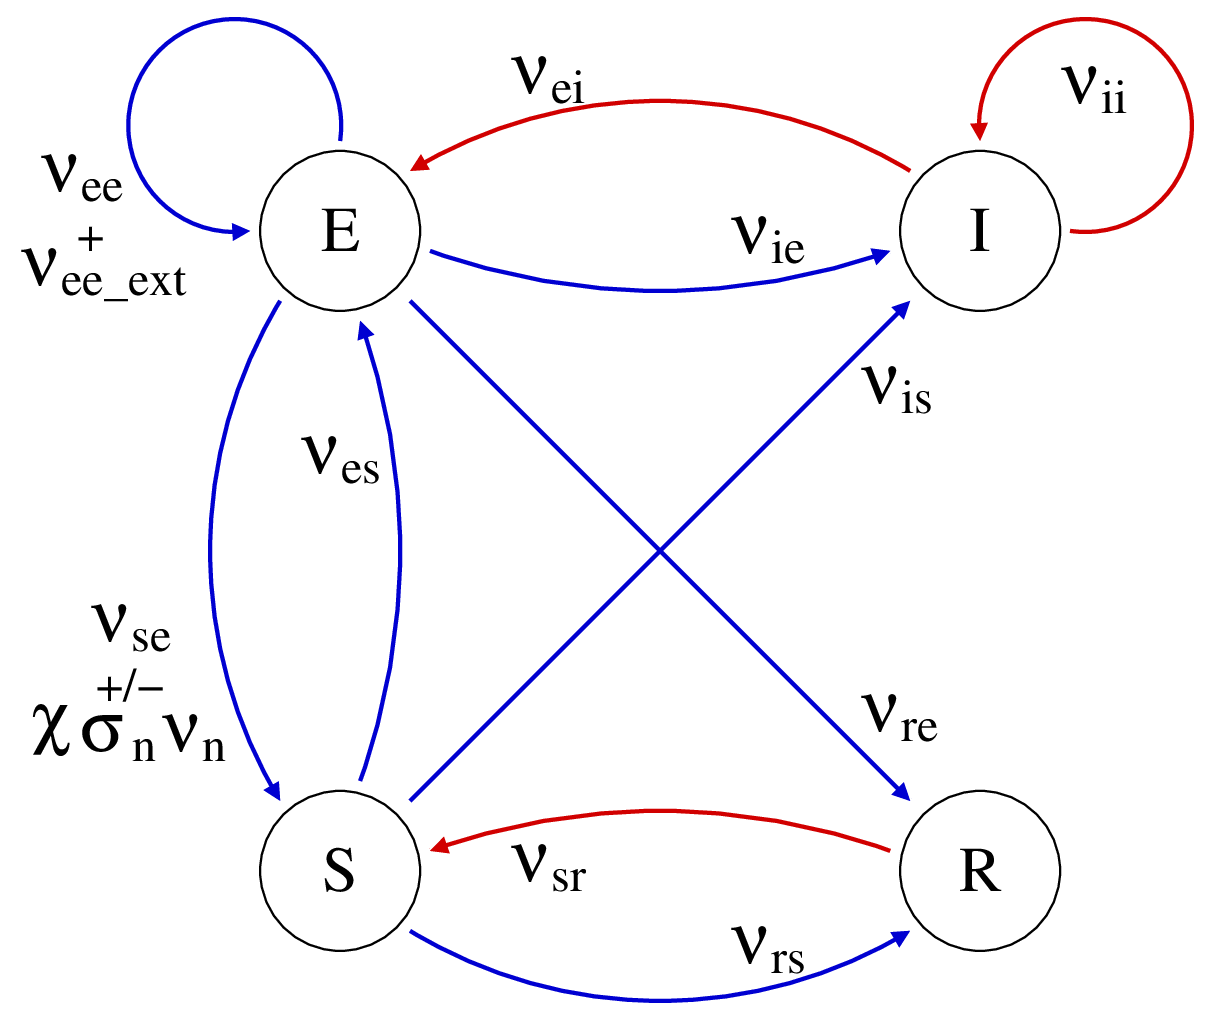
\includegraphics[height=2.5in]{figures/robinson-model-loops}}
{Simplified diagram of the extended Robinson model, showing feedback loops.}
{fig-robinson-loops}

A list of potential oscillation loops and their oscillation frequencies is
given in Table \ref{tab-robinson-loops}. For loops consisting entirely of
positive coefficients, or with two negative coefficients, the oscillation
period is the time needed to complete a single circuit. For loops with one
negative coefficient, the oscillation period is the time needed to complete
two circuits around the loop (in the same manner as a ring oscillator).
Harmonics of these oscillation frequencies are also supported.

The number of arc traversals needed for one oscillation period is noted.
Per above, this may reflect either one or two cycles around the loop. Each
arc traversal involves gain from arc coefficients (noted in the table),
small-signal gain from the $Q(V)$ transfer function (omitted from the table),
and delay from the $\alpha$ and $\beta$ filter components. Delay
contributions from the cortex excitatory population $\gamma$ filter
component and from the cortex-thalamus loop are noted in the table where
applicable.

\tabdef{%
\begin{tabular}{ccccccc}\hline
\textbf{Label} & \textbf{Arcs} & \textbf{Gamma} & \textbf{C-T Loop} &
\textbf{Period} & \textbf{Frequency} & \textbf{Coupling Gain} \\
\hline
%
EE & 1 & Y & -- & 45 ms & 22 Hz & $(\nu_{ee} + \nu_{ee\_ext})$ \\
ES & 2 & Y & Y & 150 ms & 6.7 Hz & $\nu_{se} \cdot \nu_{es}$ \\
%
ERSI & 4 & Y & Y & 200 ms & 5.0 Hz &
$\nu_{re} \cdot \nu_{sr} \cdot \nu_{is} \cdot \nu{ei}$ \\
%
\hline
%
II & 2 & -- & -- & 25 ms & 20 Hz & $\nu_{ii}$ \\
%
EI & 4 & Y & -- & 140 ms & 7 Hz & $2 \cdot \nu_{ie} \cdot \nu_{ei}$ \\
SR & 4 & -- & -- & 100 ms & 10 Hz & $2 \cdot \nu_{rs} \cdot \nu_{sr}$ \\
%
ESI & 6 & Y & Y & 350 ms & 2.9 Hz &
$2 \cdot \nu_{se} \cdot \nu_{is} \cdot \nu_{ei}$ \\
ERS & 6 & Y & Y & 350 ms & 2.9 Hz &
$2 \cdot \nu_{re} \cdot \nu_{sr} \cdot \nu_{es}$ \\
%
\hline
\end{tabular}
}{Extended Robinson model oscillation modes. Top modes: single-cycle
(non-inverting). Bottom modes: two-cycle (inverting). Activation function
gain is not shown.}
{tab-robinson-loops}

Resonant loops explicitly described in Section IV of Robinson 2002 are the
ones marked ES, ERS, and SR in Table \ref{tab-robinson-loops}. Considering
only those loops, the oscillation periods described in Section V of
Robinson 2002 are consistent with the estimated periods of the ERS and
SR loops.

The authors of Robinson 2002 were primarily concerned with noise-excited
oscillations, and so only evaluated oscillation loops that included the
specific nucleus. Evaluation was expressed in terms of the transfer
function from the noise signal (input) to the firing rate of cortex
excitatory neurons (output). Resonant oscillations were presumed to occur
at frequencies for which this transfer function diverged (producing
arbitrarily large output for finite input). This work instead considers
gain within a loop, with resonant oscillations corresponding to a loop
gain exceeding unity. As this does not explicitly consider noise excitation,
all of the loops described in Table \ref{tab-robinson-loops} may be
analyzed.

%
%
\section{Operating Points}
\label{sect-robinson-math-dc}

As was described in Robinson 2002, the dynamics of the extended Robinson
model can be analyzed by considering unchanging (DC) firing rates, and
evaluating the small-signal gain around these operating points. While this
was used to find the transfer function
$\frac{\phi_e(\omega)}{\phi_n(\omega)}$ in Robinson 2002, here it is used
to find the small-signal loop gain (to determine which oscillating modes
are dominant for given parameter values).

At a given operating point, the sensitivity of the gain of the dominant
loops to each of the $\nu_{ab}$ coefficients provides insight into which
network connections are most relevant for influencing dynamcis at that
operating point. $\nu_{ee\_ext}$ is particularly of interest, as this
may be used as a proxy for the sensitivity of network dynamics to changes
in the connectivity matrix between different excitatory cortex neuron
populations.

For time-independent operating point analysis, Equation
\ref{eq-robinson-potential} reduces to:

\begin{equation}
V_a = \sum_b \nu_{ab} \phi_b
\label{eq-robinson-dc-potential}
\end{equation}

Equation \ref{eq-robinson-sigmoid} (defining $Q(V)$) is unchanged, and
Equation \ref{eq-robinson-gamma} reduces to:

\begin{equation}
\phi_a = Q(V_a)
\label{eq-robinson-dc-nogamma}
\end{equation}

Combining Equations \ref{eq-robinson-dc-potential} and
\ref{eq-robinson-dc-nogamma} gives:

\begin{equation}
V_a = \sum_b \nu_{ab} Q(V_b)
\label{eq-robinson-dc-scalar}
\end{equation}
%
\begin{equation}
\vec{V} = \mathbf{N} Q(\vec{V})
\label{eq-robinson-dc-vector}
\end{equation}

In Equation \ref{eq-robinson-dc-vector}, vector $\vec{V}$ contains as its
elements all $V_a$, matrix $\mathbf{N}$ contains as its elements all
$\nu_{ab}$, and the activation function Q acts separately on each element
of $\vec{V}$.

The activation function given in \ref{eq-robinson-sigmoid-prime} can be
rewritten as:

\begin{equation}
Q(V) = \frac{Q_{max}}{1 +
e^{\left ( \frac{V_{th}}{\sigma'_{th}} \right )}
e^{- \left ( \frac{V}{\sigma'_{th}} \right )}
}
\label{eq-robinson-sigmoid-shuffle-1}
\end{equation}

For firing rates that are much less than $Q_{max}$ (such as those plotted
in Robinson 2002), the exponential term dominates, and the activation
function can be approximated as:

\begin{equation}
Q(V) \approx Q_{max} \, e^{- \left ( \frac{V_{th}}{\sigma'_{th}} \right )}
e^{\left ( \frac{V}{\sigma'_{th}} \right )}
\label{eq-robinson-sigmoid-approx-full}
\end{equation}
%
\begin{equation}
Q(V) \approx Q_0 \, e^{\left ( \frac{V}{\sigma'_{th}} \right )}
\label{eq-robinson-sigmoid-approx}
\end{equation}
%
\begin{equation}
Q_0 = Q_{max} \, e^{- \left ( \frac{V_{th}}{\sigma'_{th}} \right )}
\label{eq-robinson-sigmoid-q0}
\end{equation}

The operating point equation then becomes Equation
\ref{eq-robinson-dc-vector-approx}, where exponentiation is performed
separately for each element of $\vec{V}$:

\begin{equation}
\vec{V} \approx
\mathbf{N} \, Q_0 \, e^{\left ( \frac{\vec{V}}{\sigma'_{th}} \right )}
\label{eq-robinson-dc-vector-approx}
\end{equation}

This system of exponential equations may be solved numerically.

Alternatively, a system of linear equations may be obtained by assuming
that potentials are small compared to $\sigma'_{th}$.
\textbf{This is not a robust assumption;} it is used as an estimate only.
With this caveat kept in mind, a linear approximation of the exponential
function may be used (the first-order Taylor expansion), giving the following
(where $\vec{1}$ denotes a vector where all elements are unity):

\begin{equation}
\vec{V} \approx \mathbf{N} \, Q_0 \,
\left [ \vec{1} + \left ( \frac{1}{\sigma'_{th}} \right ) \vec{V} \right ]
\end{equation}
%
\begin{equation}
\left ( \frac{1}{Q_0} \right ) \vec{V} \approx \mathbf{N} \, \vec{1}
+ \left ( \frac{1}{\sigma'_{th}} \right ) \mathbf{N} \, \vec{V}
\end{equation}
%
\begin{equation}
\left [ \left ( \frac{1}{Q_0} \right ) \mathbf{I}
- \left ( \frac{1}{\sigma'_{th}} \right ) \mathbf{N}
\right ] \vec{V} \approx \mathbf{N} \, \vec{1}
\label{eq-robinson-dc-vector-linear}
\end{equation}

Equation \ref{eq-robinson-dc-vector-linear} has the form
$\mathbf{A} \vec{V} = \vec{b}$, and so may be solved as a set of linear
equations. The operating point estimated using Equation
\ref{eq-robinson-dc-vector-linear} \textbf{must} be examined to confirm
that $|V_a| \ll \sigma'_{th}$ for all $V_a$. If this constraint does not
hold, the estimate is not correct.

As a representative example, Table \ref{tab-robinson-operating-point} shows
the operating point corresponding to the model parameters given in Table
\ref{tab-robinson-params} and the coupling coefficients given in Table
\ref{tab-robinson-couplings}. A single population was considered (no
$\nu_{ee\_ext}$ coupling). All of the operating point values satisfy the
constraint for exponential approximation validity ($\phi \ll 250$), and
while the constraint for linear approximation is not satisfied
($V \ll 3.3$), they are sufficiently close to the desired domain that the
linear approximation result can be used as a seed value for obtaining the
exponential approximation result via gradient descent.

\tabdef{%
\begin{tabular}{c|cccc}
\hline
 & \textbf{Measured} & \textbf{Exponential} & \textbf{Linear} & \\
\hline
$\phi_e$ & 4.2 & 4.1 & 4.8 & /sec \\
$\phi_i$ & 4.2 & 4.1 & 4.8 & /sec \\
$\phi_s$ & 3.3 & 3.2 & 4.0 & /sec \\
$\phi_r$ & 5.3 & 5.3 & 5.6 & /sec \\
\hline
$V_e$ & 1.51 & 1.44 & 2.01 & mV \\
$V_i$ & 1.51 & 1.44 & 2.01 & mV \\
$V_s$ & 0.75 & 0.66 & 1.41 & mV \\
$V_r$ & 2.34 & 2.31 & 2.49 & mV \\
\hline
\end{tabular}
}{Measured and estimated operating points for a representative model.
``Measured'' values were averaged over a 30-second simulation window.
``Exponential'' and ``linear'' values were estimated using Equations
\ref{eq-robinson-dc-vector-approx} (using gradient descent) and
\ref{eq-robinson-dc-vector-linear} (as a system of linear equations),
respectively.}
{tab-robinson-operating-point}

%
%
\section{Small-Signal Gain and Dominant Oscillations}
\label{sect-robinson-math-gain}

The small-signal gain $G_{ab}$ of any given arc is the derivative of its
output firing rate with respect to its input firing rate. For oscillations
with frequencies much lower than the $\alpha$, $\beta$, and $\gamma$ filter
corner frequencies, this may be estimated by taking the derivative of the
DC operating point equations (rather than requiring an analysis of the full
system dynamics):

\begin{equation}
G_{ab} = \frac{d\phi_a}{d\phi_b}
\approx \frac{d}{d\phi_b} \left [ Q(V_a) \right ]
\end{equation}
%
\begin{equation}
G_{ab} \approx Q'(V_a) \frac{dV_a}{d\phi_b}
\end{equation}
%
\begin{equation}
G_{ab} \approx
Q'(V_a) \frac{d}{d\phi_b} \left [ \sum_c \nu_{ac} \phi_c \right ]
\end{equation}
%
\begin{equation}
G_{ab} \approx Q'(V_a) \nu_{ab}
\label{eq-robinson-gain-qprime}
\end{equation}

The sigmoid response function is defined in terms of the logistic function:

\begin{equation}
\left \{
\begin{array}{l}
Q(V) = Q_{max} L \left (\frac{V - V_{th}}{\sigma'_{th}} \right ) \\
\\
L(x) = \frac{1}{1 + e^{-x}} = \frac{e^x}{1 + e^x} \\
\\
\sigma'_{th} = \frac{\sqrt{3}}{\pi}\sigma_{th} \\
\end{array}
\right .
\label{eq-robinson-sigmoid-logistic}
\end{equation}

The derivative of the logistic function is:

\begin{equation}
L'(x) = L(x) \left ( 1 - L(x) \right ) = \frac{e^x}{(1 + e^x)^2}
\label{eq-robinson-logistic-derivative}
\end{equation}

This gives the derivative of the sigmoid response function:

\begin{equation}
Q'(V) = Q_{max} L' \left ( \frac{V - V_{th}}{\sigma'_{th}} \right )
\frac{d}{dV} \left [ \frac{V - V_{th}}{\sigma'_{th}} \right ]
\end{equation}
%
\begin{equation}
Q'(V) = \frac{Q_{max}}{\sigma'_{th}}
L' \left ( \frac{V - V_{th}}{\sigma'_{th}} \right )
\end{equation}
%
\begin{equation}
Q'(V) = \frac{Q_{max}}{\sigma'_{th}}
L \left ( \frac{V - V_{th}}{\sigma'_{th}} \right )
\left ( 1 - L \left ( \frac{V - V_{th}}{\sigma'_{th}} \right ) \right )
\end{equation}
%
\begin{equation}
Q'(V) = \frac{Q_{max}}{\sigma'_{th}}
L \left ( \frac{V - V_{th}}{\sigma'_{th}} \right )
\left ( 1 - \frac{Q_{max}}{Q_{max}}
L \left ( \frac{V - V_{th}}{\sigma'_{th}} \right ) \right )
\end{equation}
%
\begin{equation}
Q'(V) = \frac{1}{\sigma'_{th}} Q(V) \left ( 1 - \frac{Q(V)}{Q_{max}} \right )
\label{eq-robinson-sigmoid-derivative}
\end{equation}

Combining this with Equation \ref{eq-robinson-gain-qprime} gives:

\begin{equation}
G_{ab} \approx \frac{\nu_{ab}}{\sigma'_{th}}
Q(V_a) \left ( 1 - \frac{Q(V_a)}{Q_{max}} \right )
\end{equation}
%
\begin{equation}
G_{ab} \approx \frac{\nu_{ab}}{\sigma'_{th}}
\phi_a \left ( 1 - \frac{\phi_a}{Q_{max}} \right )
\label{eq-robinson-gain}
\end{equation}

This is Equation 10 from Robinson 2002.

The small-signal gain of a loop at low frequencies is the product of
$G_{ab}$ for each arc in the loop (as with the $S_d$, $S_i$, and $S_r$
values in section IV of Robinson 2002).
At frequencies that approach the low-pass filter cutoffs described in
Section \ref{sect-robinson-math-lowpass}, Equation
\ref{eq-robinson-lowpass-albet} must be applied to attenuate each edge, and
Equation \ref{eq-robinson-lowpass-gamma} must be applied to attenuate any
edge leaving the excitatory cortex population node.
The small-signal gains for the loops in Table \ref{tab-robinson-loops} are
shown in Table \ref{tab-robinson-loopgain}. These were evaluated at the
exponential approximation operating point from
Table \ref{tab-robinson-operating-point}, with low-pass filter attenuation
applied.

\tabdef{%
\begin{tabular}{ccccc} \hline
\textbf{Label} & \textbf{Frequency} & \textbf{Cycle Time} &
\textbf{Cycle Gain} & \textbf{Envelope Tau} \\ \hline
%
EE & 22 Hz & 45 ms & 0.14 & -23 ms \\
II & 20 Hz & 25 ms & -0.68 & -66 ms \\ \hline
%
EI & 7.1 Hz & 70 ms & -1.39 & \textbf{210 ms} \\
ES & 6.7 Hz & 150 ms & 0.81 & -690 ms \\
SR & 10.0 Hz & 50 ms & -0.09 & -20 ms \\ \hline
%
ESI & 2.9 Hz & 175 ms & -2.93 & \textbf{163 ms} \\
ERS & 2.9 Hz & 175 ms & -0.56 & -300 ms \\ \hline
%
ERSI & 5.0 Hz & 200 ms & 0.68 & -520 ms \\ \hline
%
\end{tabular}
}{Small-signal gains of extended Robinson model oscillation modes. Positive
gains correspond to single-cycle loops; negative gains to two-cycle loops.
Gains with absolute values smaller than 1 correspond to damped loops; gains
with absolute values greater than 1 correspond to oscillation modes that
grow over time with time constant $\tau_{loop}$.}
{tab-robinson-loopgain}

The single-cycle delay and single-cycle gain in a loop together define a time
constant over which that loop's oscillation's envelope grows or decays,
per Equations \ref{eq-robinson-gaintau} and \ref{eq-robinson-envtau}.
An envelope time constant that is positive indicates that an oscillation
mode grows with time; the smaller the time constant, the faster the growth:

\begin{equation}
| G_{loop} | = e^{\left ( \frac{t_{loop}}{\tau_{env}} \right )}
\label{eq-robinson-gaintau}
\end{equation}
%
\begin{equation}
\tau_{env} = \frac{t_{loop}}{\ln | G_{loop} |}
\label{eq-robinson-envtau}
\end{equation}

The dominant oscillation modes are expected to be those with the shortest
positive envelope time constants. Only two such loops are present with the
parameters from Tables \ref{tab-robinson-params} and
\ref{tab-robinson-couplings}: The EI loop in the cortex (at 7 Hz) and the
ESI loop through the thalamus (at 3 Hz). The gain in the ESI loop may
fluctuate due to the $\chi \sigma_n \nu_n$ contribution to $\nu_{se}$ (shown
in Figure \ref{fig-robinson-loops}). A power spectrum from a simulation
using these parameters is shown in Figure \ref{fig-robinson-spectrum},
showing a clear peak at 8 Hz (near the predicted EI loop resonance).

\figdef{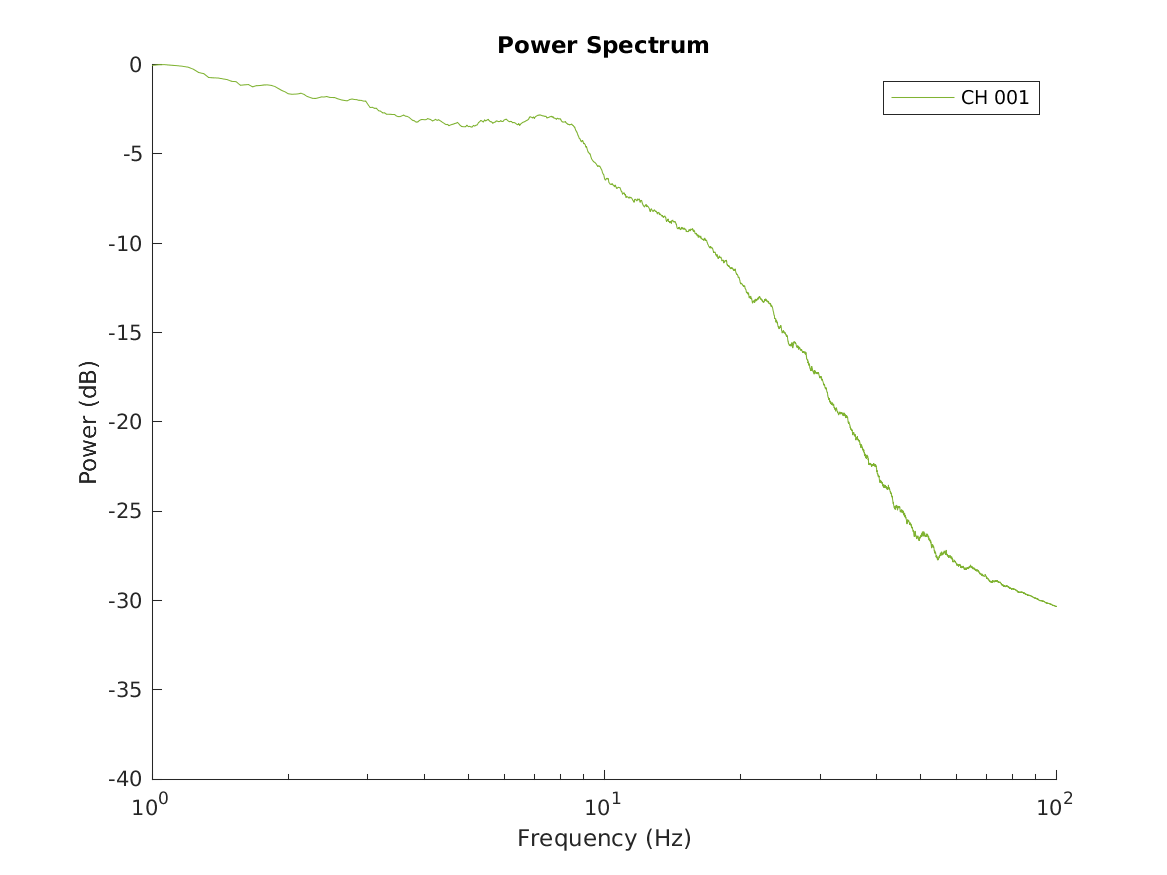
\includegraphics[height=3in]{plots/20240108/spectrum-hindriks}}
{Power spectrum from a Robinson model simulation.}
{fig-robinson-spectrum}

%
%
\section{Adjusting Gain by Tuning Coupling Coefficients}
\label{sect-robinson-math-tuning}
%
% FIXME - Convenience macro.
\newcommand{\deln}{\nabla_{\mathbf{N}}}

Tuning the behavior of the simulated system is done by adjusting the
internal coupling coefficients $\nu_{ab}$ (aggregated as matrix
$\mathbf{N}$). The goal is typically to cause specific oscillation modes
to become dominant. To facilitate this, the sensitivity of loop gain with
respect to the coupling coefficients may be evaluated by computing the
gradient of gain with respect to $\mathbf{N}$.

The gain across a given network edge may be expressed in terms of the
edge's coupling coefficient and the derivative of the activation function,
per Equations \ref{eq-robinson-gain-qprime} and
\ref{eq-robinson-sigmoid-derivative}:

\begin{equation}
G_{ab} \approx \nu_{ab} \, Q'(V_a)
\end{equation}
%
\begin{equation}
Q'(V_a) = \frac{1}{\sigma'_{th}} \phi_a
\left ( 1 - \frac{\phi_a}{Q_{max}} \right )
\end{equation}

Taking the gradient with respect to $\mathbf{N}$ gives:

\begin{equation}
\deln G_{ab} \approx Q'(V_a) \deln \nu_{ab} + \nu_{ab} \deln Q'(V_a)
\label{eq-robinson-gain-gradient}
\end{equation}

$\deln \nu_{ab}$ is a matrix whose elements are zero except for a single
element at row $a$ column $b$, which is unity. The gradient of $Q'(V_a)$ is:

\begin{equation}
\deln Q'(V_a) = \deln \left [
\frac{1}{\sigma'_{th}} \phi_a \left ( 1 - \frac{\phi_a}{Q_{max}} \right )
\right ]
\end{equation}
%
\begin{equation}
\deln Q'(V_a) =
\frac{1}{\sigma'_{th}} \left (
\left ( 1 - \frac{\phi_a}{Q_{max}} \right ) \deln \phi_a
+ \phi_a \deln \left [ 1 - \frac{\phi_a}{Q_{max}} \right ]
\right )
\end{equation}
%
\begin{equation}
\deln Q'(V_a) = \frac{1}{\sigma'_{th}}
\left ( 1 - 2 \frac{\phi_a}{Q_{max}} \right ) \deln \phi_a
\label{eq-robinson-qprime-gradient}
\end{equation}

In principle, the gradient of the firing rate $\deln \phi_a$ may be
evaluated by taking the gradient with respect to $\mathbf{N}$ of Equations
\ref{eq-robinson-sigmoid-approx} and \ref{eq-robinson-dc-vector-approx}. In
practice, the firing rate gradients are evaluated numerically by finding an
operating point and making small perturbations to each $\nu_{ab}$.

The gradient of the gain along a path consisting of multiple edges can be
computed using the product rule. For two-, three-, and four-edge loops,
this gives:

\begin{equation}
\deln [ G_{ab} G_{ba} ] =
( \deln [ G_{ab} ] ) G_{ba} + G_{ab} ( \deln [ G_{ba} ] )
\label{eq-robinson-loop2-gain-gradient}
\end{equation}
%
\begin{equation}
\deln [ G_{ab} G_{bc} G_{ca} ] =
( \deln [ G_{ab} ] ) G_{bc} G_{ca} + G_{ab} ( \deln [ G_{bc} ] ) G_{ca}
+ G_{ab} G_{bc} ( \deln [ G_{ca} ] )
\label{eq-robinson-loop3-gain-gradient}
\end{equation}
%
\begin{equation}
\begin{array}{c}
\deln [ G_{ab} G_{bc} G_{cd} G_{da} ] =
( \deln [ G_{ab} ] ) G_{bc} G_{cd} G_{da}
+ G_{ab} ( \deln [ G_{bc} ] ) G_{cd} G_{da}
\\
+ G_{ab} G_{bc} ( \deln [ G_{cd} ] ) G_{da}
+ G_{ab} G_{bc} G_{cd} ( \deln [ G_{da} ] )
\end{array}
\label{eq-robinson-loop4-gain-gradient}
\end{equation}

While Equations \ref{eq-robinson-loop2-gain-gradient} through
\ref{eq-robinson-loop4-gain-gradient} can be expanded and written in terms
of $\nu_{ab}$, $\phi_{a}$, and $\deln \phi_{a}$, it is not particularly
useful to do so (since with or without such expansion the gradient will
have to be evaluated numerically).

Plots of the gradients of the loop gains of the EI and ESI loops (from
Table \ref{tab-robinson-loopgain}) are shown in Figure
\ref{fig-robinson-loopgrad}. The ``raw'' gradients are the change in loop
gain with respect to each of the $\nu_{ab}$ coupling weights (i.e.
$\deln G_{loop}$). The ``normalized'' gradients are divided by $G_{loop}$,
to show the \textit{relative} change in loop gain resulting from changes
to $\nu_{ab}$. In particular, this flips the sign of the gradient for
loop gains that are negative (with a positive normalized gradient indicating
that the loop gain is getting \textit{larger}, not more positive).

\figdef{%
\begin{tabular}{cc}
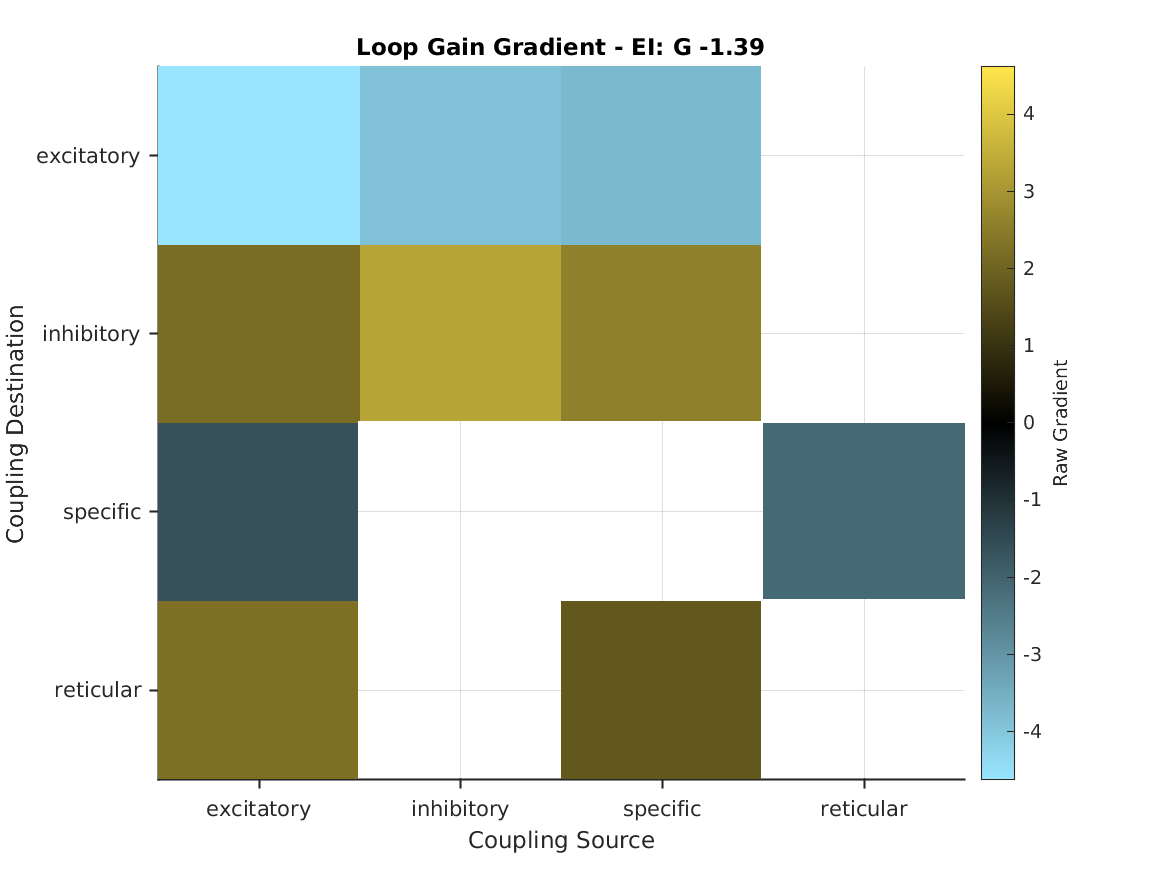
\includegraphics[height=2in]{plots/20240110/grad-loop-EI-raw} &
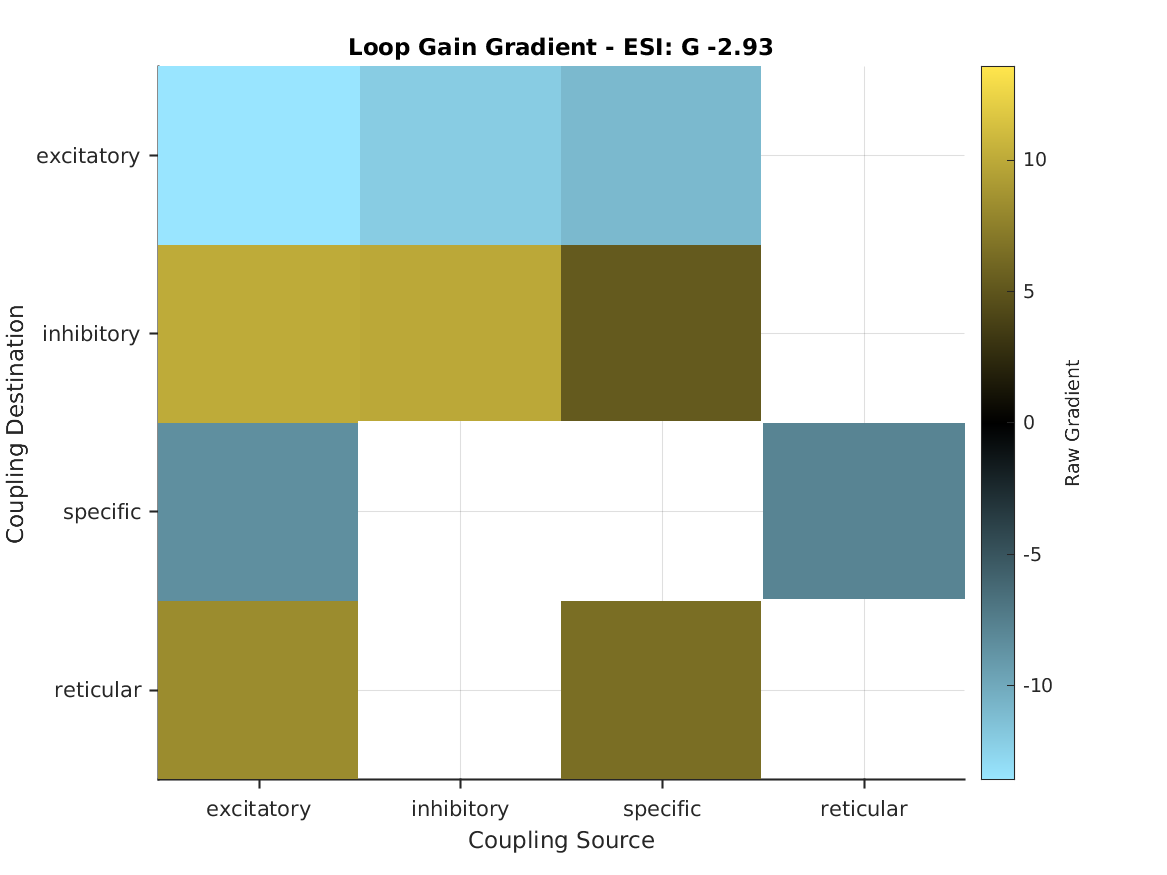
\includegraphics[height=2in]{plots/20240110/grad-loop-ESI-raw} \\
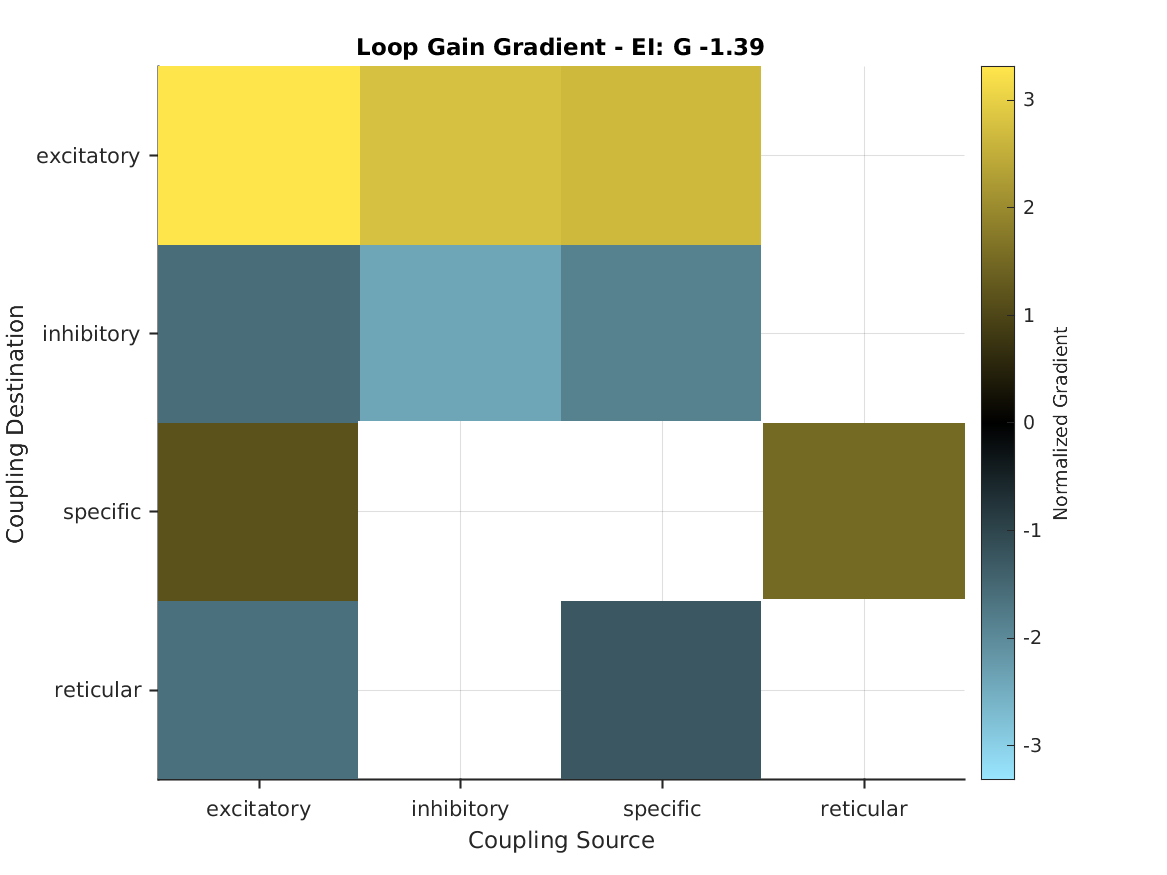
\includegraphics[height=2in]{plots/20240110/grad-loop-EI-norm} &
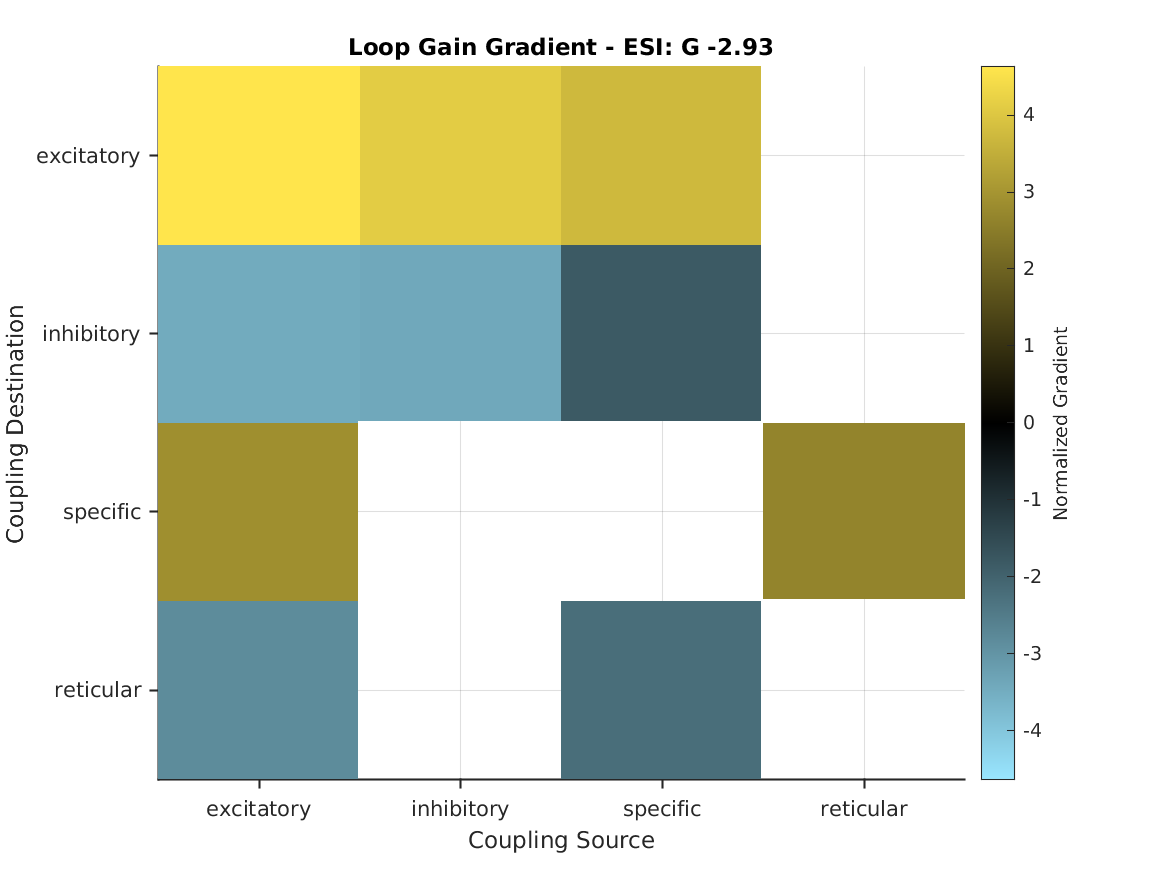
\includegraphics[height=2in]{plots/20240110/grad-loop-ESI-norm} \\
\end{tabular}
}{Gradient of loop gain with respect to $\nu_{ab}$, for the EI loop (left)
and the ESI loop (right). Top row: raw gradient. Bottom row: normalized
gradient (gradient divided by $G_{loop}$).}
{fig-robinson-loopgrad}

The gradients may be visually inspected to gain a qualitative understanding
of which $\nu_{ab}$ coupling weights have substantial impact on which loops.
In particular, sensitivity to the strength of the $\nu_{ee}$ coupling in this
analysis indicates sensitivity to the strength of the $\nu_{ee\_ext}$
coupling between populations, and to the weights in the population mixing
matrix.

Inspection of the gradient plots may also guide hand-tuning of coupling
weights. The main qualitative take-away is that while there are typically
a small number of $\nu_{ab}$ coupling weights that most strongly affect a
given loop, any given weight affects many loops, so weights must be jointly
optimized against all loop gains rather than optimized individually against
a single loop gain.

The gradients may also be used as the basis of gradient-guided searches of
parameter space. In practice, the gradient may not need to be explicitly
computed for this, since optimization library functions such as
\texttt{fsolve} may compute it numerically themselves by sampling the
loop gain.


\fixme{Show how to find regions of parameter space where desired loops are
dominant, including ones where the mixing matrix matters. Show where the
regions Robinson plotted are. Show where the region Hindriks used is.}

%
%
% This is the end of the file.

%
%
\end{document}

%
% This is the end of the file.
